% ============================================================
% 4.4 SELECTION (first part) -- Writer: Ignacio Gimeno -- about 230 words
% Numbers: results/weighted_selection_by_field.csv, results/final_figures_stats.json
% (fig4), figures/final/CAPTIONS.md (entry fig4). Outline entries 8 [now 9] and 9a.
% Pablo's paragraph on the normal-approximation checks follows (04f).
% ============================================================

\subsection{A Single Raw-GPA Ranking Gives Unequal Access}
\label{sec:res-selection}

\guide{Ignacio -- Paragraph: Figure~\ref{fig:selection}}{%
\textbf{Claim (outline 9):} a single raw-GPA ranking gives very unequal access by field.\\
\textbf{Numbers:} in the median university-year, 41\% of Nursing graduates reach the top 20\% against 6\% of Business administration graduates (interquartile ranges 29--54\% and 2--13\%); 664 university-years, 79 universities.\\
\textbf{Must say (CAPTIONS.md):} these shares are simulated from published means and quartiles (\S\ref{sec:methods-simulation}), not observed selections.\\
\textbf{Interpretation:} with equal access every field would send 20\%; the field a student chose changes their chance of selection several times over.}
\budget{150}{Ignacio}

\begin{figure}[t]
  \centering
  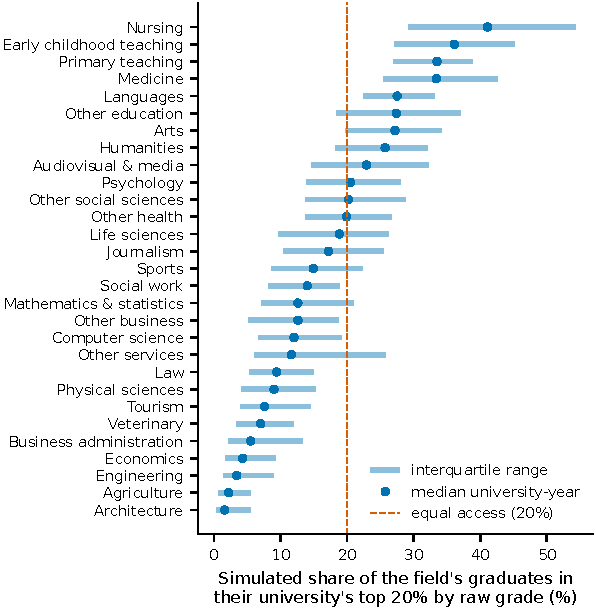
\includegraphics[width=\linewidth]{fig4_selection}
  \caption{\capguide{Ignacio -- see CAPTIONS.md, entry "Figure 4" (file fig4): simulated, not observed; normal approximation from mean and quartiles; graduate-weighted top-20\% cut per university-year; 664 university-years; median and interquartile range; dashed red line = equal access.}}
  \label{fig:selection}
\end{figure}
